\begin{figure}[htb]
\vspace{-0.1cm}
    \begin{center}
    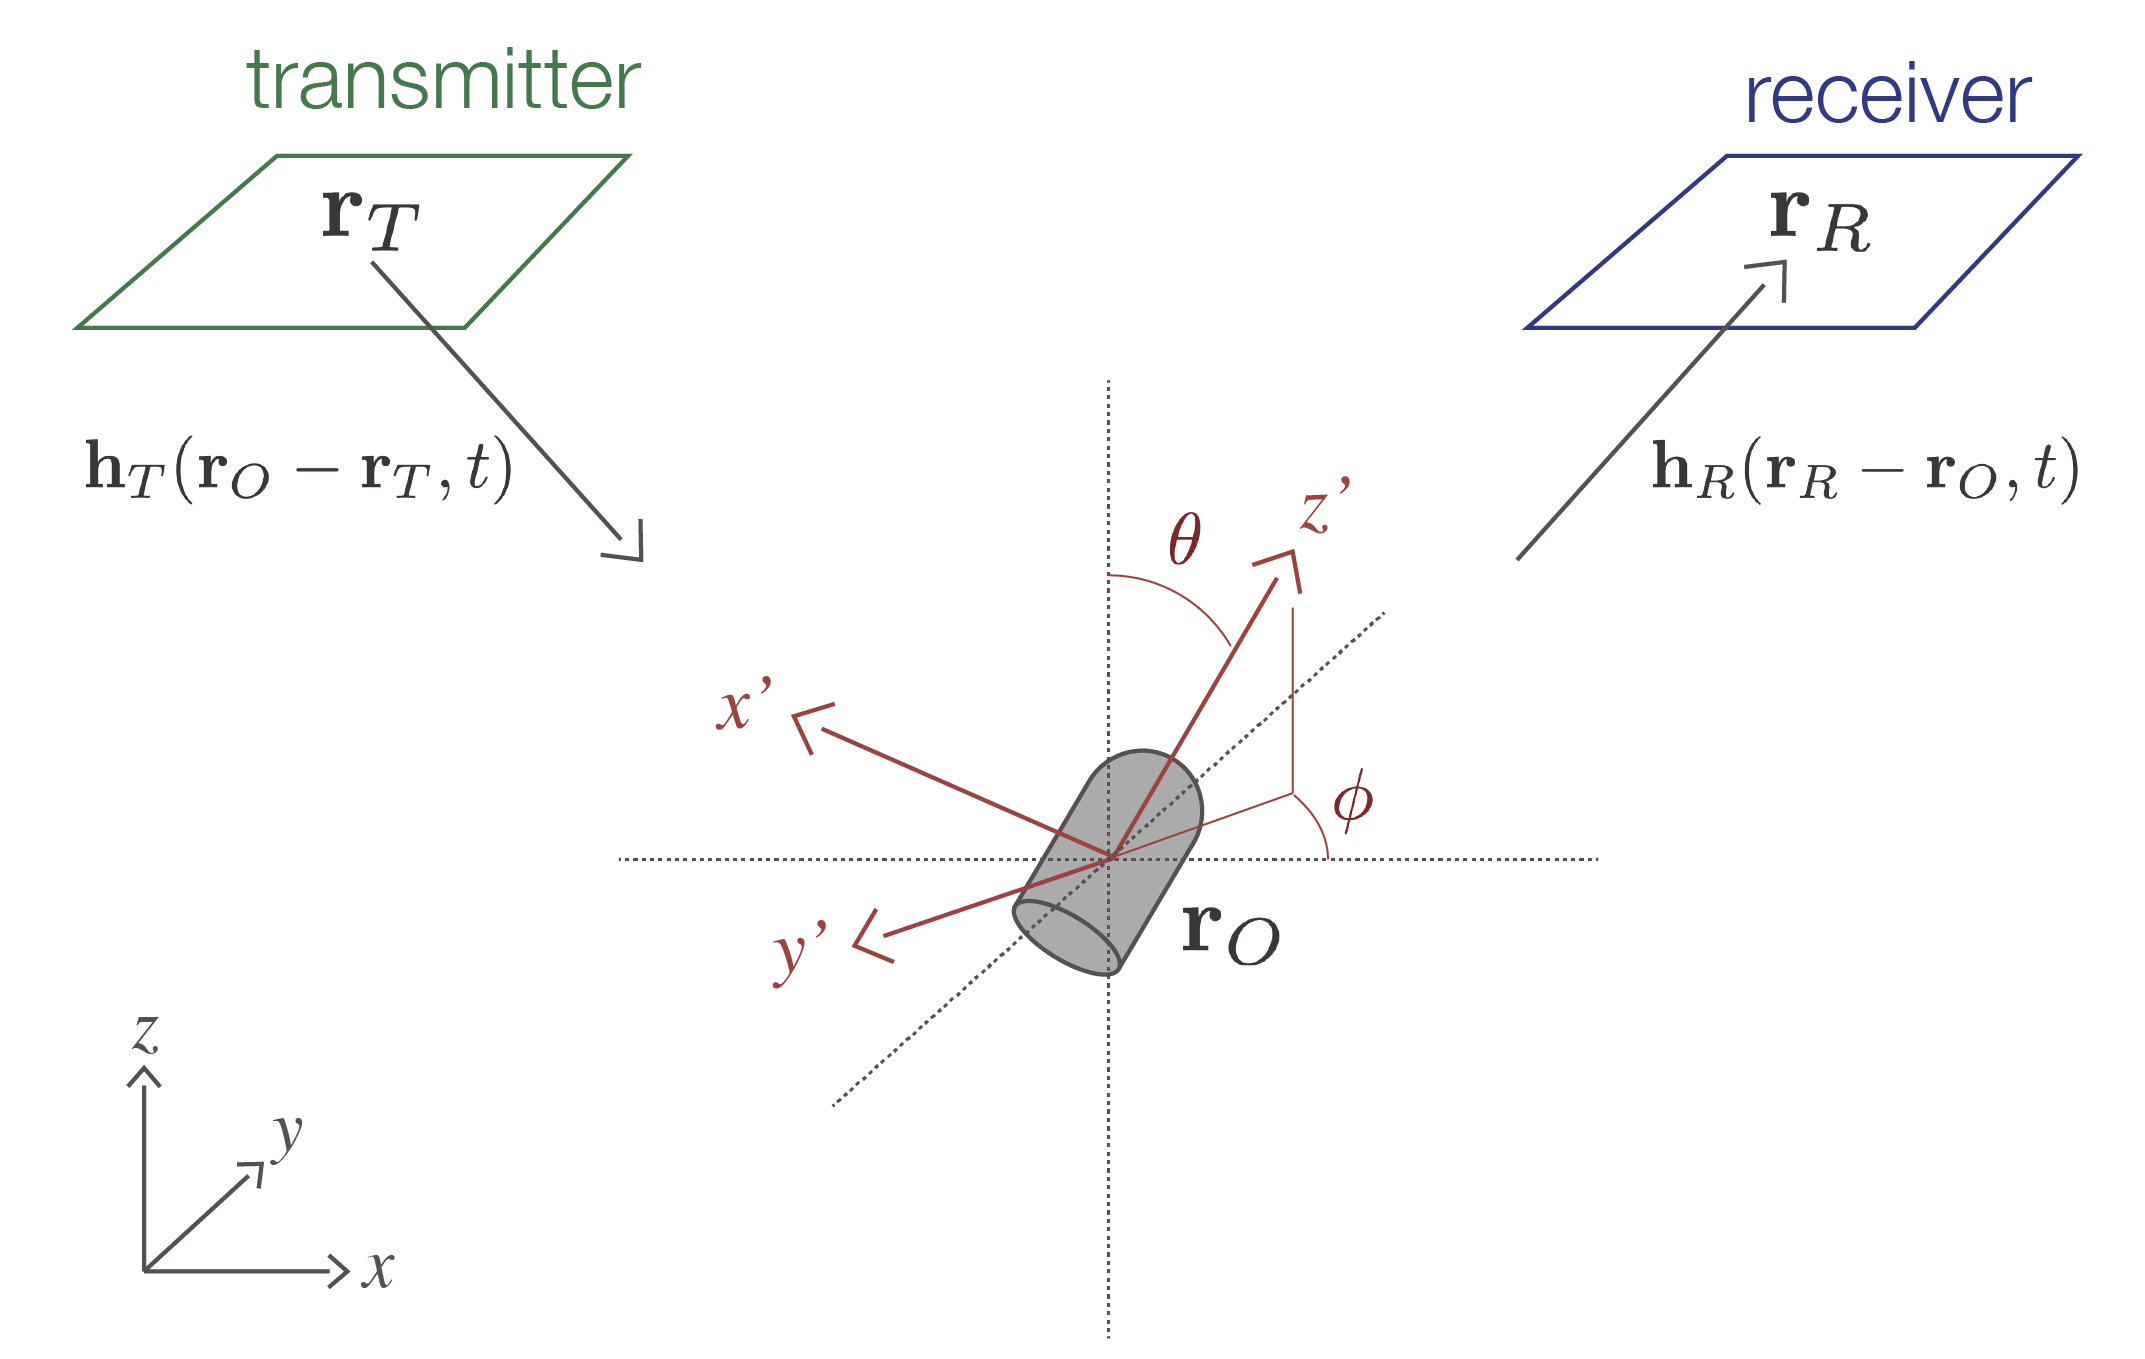
\includegraphics[width=0.85\columnwidth]{figures/uxo-coordinates-01-01.png}
    \end{center}
    \vspace{-0.5cm}
\caption{
    Electromagnetic experiment to detect a UXO.
    The transmitter produces a primary magnetic field which excites
    currents in a conductive UXO producing a secondary magnetic field
    which is measured at the receiver.
}
\label{fig:uxo-coordinates}
\vspace{-0.1cm}
\end{figure}
